\documentclass[tikz,border=3.14mm]{standalone}
\usetikzlibrary{positioning,chains}
\begin{document}
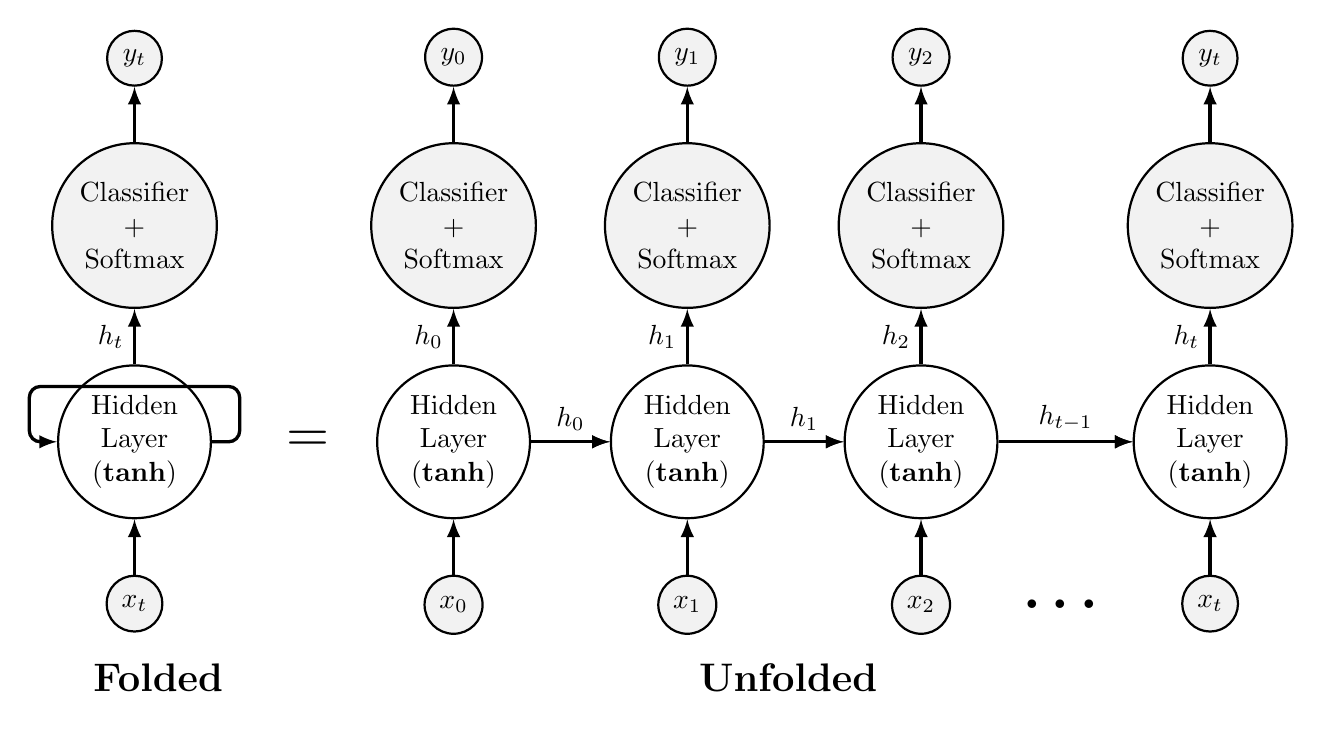
\begin{tikzpicture}[item/.style={circle,draw,thick,align=center},
itemc/.style={item,on chain,join}]
 \begin{scope}[start chain=going right,nodes=itemc,every
 join/.style={-latex,very thick},local bounding box=chain]
 \path node (A0) {Hidden\\ Layer\\ (\textbf{tanh})} node (A1) {Hidden\\ Layer\\ (\textbf{tanh})} node (A2) {Hidden\\ Layer\\ (\textbf{tanh})} node[xshift=2em] (At)
 {Hidden\\ Layer\\ (\textbf{tanh})};
 \end{scope}
 \node[left=1em of chain,scale=2] (eq) {$=$};
 \node[left=2em of eq,item] (AL) {Hidden\\ Layer\\ (\textbf{tanh})};
 \path (AL.west) ++ (-1em,2em) coordinate (aux);
 \draw[very thick,-latex,rounded corners] (AL.east) -| ++ (1em,2em) -- (aux) 
 |- (AL.west) node[pos=0.25,above right] {};
 \foreach \X in {0,1,2,t} 
 {\draw[very thick,-latex] (A\X.north) -- ++ (0,2em)
 node[above,item,fill=gray!10] (h\X) {Classifier\\ +\\ Softmax} node[midway,left] {$h_\X$};

 \draw[very thick,-latex] (h\X.north) -- ++ (0,2em)
 node[above,item,fill=gray!10] (C\X) {$y_\X$} node[midway,left] {};
 
 \draw[very thick,latex-] (A\X.south) -- ++ (0,-2em)
 node[below,item,fill=gray!10] (x\X) {$x_\X$} node[midway,left] {};}
 \draw[white,line width=0.8ex] (AL.north) -- ++ (0,1.9em);
 \draw[very thick,-latex] (AL.north) -- ++ (0,2em)
 node[above,item,fill=gray!10] (hL){Classifier\\ +\\ Softmax} node[midway,left] {$h_t$};

  \draw[very thick,-latex] (hL.north) -- ++ (0,2em)
 node[above,item,fill=gray!10] {$y_t$} node[midway,left] {};

 \draw[very thick,latex-] (AL.south) -- ++ (0,-2em)
 node[below,item,fill=gray!10] {$x_t$} node[midway,left] {};
 \path (x2) -- (xt) node[midway,scale=2,font=\bfseries] {\dots};
 \foreach \X/\Y/\L in {A0/A1/h_0, A1/A2/h_1, A2/At/h_{t-1}} {
    \draw[very thick,-latex] (\X) -- (\Y) node[midway,above] {$\L$};
 }

\node at (-3.75,-3) {\Large\textbf{Folded}};

\node at (4.25,-3) {\Large\textbf{Unfolded}};
\end{tikzpicture}
\end{document}

